\documentclass{xjtureport}
% =============================================
% Part 0 Edit the info
% =============================================

\major{生物工程}
\name{饭饭}
\title{本科实验报告}
\stuid{2182333333}
\college{生命学院}
\date{\zhtoday}
\lab{寝室}
\course{数字信号处理}
\instructor{Hao}
\grades{59}
\expname{系统传输函数零极点分析}
\exptype{设计实验}
\partner{Bob}

\begin{document}
% =============================================
% Part 1 Header
% =============================================
\makecover
\makeheader

% =============================================
% Part 2 Main document
% =============================================

\section{实验目的和要求}
系统差分方程和传输函数是线性系统的重要概念,通过分析系统差分方程和传输函数的特性,编程查看系统零极点分布,加深对线性系统的了解。
\section{实验内容和步骤}

\subsection{实验内容}

给出如下差分方程:
$$y(n) - (0.5+a)\times y(n-1) + 0.5ay(n-2) = x(n)$$
%% 这里也可以使用 `subsubsection`
\begin{enumerate}
    \item 求解系统传输函数表达式。
    \item 当 $a$ 取 $0.8, 0.9, 1.0, 1.1$时,画出零极点分布图。
          \label{item:val}
    \item 根据 \ref{item:val} 中 $a$ 的取值,分别画出幅频响应函数图像。
\end{enumerate}

\subsection{实验步骤}
\begin{enumerate}
    \item 编写程序,求解零极点
    \item 画出图形。
    \item 观察结果。
\end{enumerate}

\section{主要仪器设备}
计算机,Matlab 软件

\section{操作方法和实验步骤}
\subsection{传输函数}
对差分方程进行处理,求出传输函数表达式。
\subsection{零极点分布图}
在此基础上,使用 Matlab 中的 \texttt{zplane} 函数进一步画出在不同 $a$ 取值情况下的零极点分布图。
\subsection{幅频响应}
之后使用 \texttt{freqz} 函数画出不同a取值情况下的频率响应图像。

\section{实验数据记录和处理}
\subsection{传输函数}
根据差分方程,传输函数如下:
$$H(z) = \frac{Y(z)}{X(z)} = \frac{z^2}{z^2-(0.5+a)z+0.5a}$$
\subsection{零极点分布图}
$a = 0.8, 0.9, 1.1$时,系统的零极点分布图及程序如下:
\begin{enumerate}
    \item 图像如图~\ref{fig:dist} 所示。
          \begin{figure}[!htbp]
              \centering
              \includegraphics[width=0.6\linewidth]{01.jpg}
              \caption{系统的零极点分布图}
              \label{fig:dist}
          \end{figure}
    \item 代码
          \lstinputlisting[language=MATLAB]{code/do.m}
\end{enumerate}

\subsection{频率响应}
$a = 0.8, 0.9, 1.0, 1.1$时,系统的频率响应函数图形及程序如下:
\begin{enumerate}
    \item 图像如图~\ref{fig:resp} 所示。
          \begin{figure}[!htbp]
              \centering
              \includegraphics[width=0.6\linewidth]{02-1.jpg}
              \caption{系统的频率响应函数图形}
              \label{fig:resp}
          \end{figure}
    \item 代码
          \lstinputlisting[language=MATLAB]{code/next.m}
\end{enumerate}

\section{实验结果与分析}

Lorem ipsum dolor sit amet, consectetur adipiscing elit. Cras sit amet pharetra orci. Pellentesque ex est, ultricies non viverra sed, iaculis sed est. Suspendisse ex felis, aliquam et nulla in, vehicula gravida velit. In porttitor volutpat tincidunt. Aenean eleifend non augue sit amet ultrices. Proin rutrum odio vitae est luctus, eu facilisis leo dapibus. Aliquam commodo efficitur erat, sit amet pulvinar nulla ultrices ac. Vestibulum ullamcorper malesuada odio. Suspendisse id sollicitudin arcu. Nam fringilla commodo neque quis posuere. Sed lobortis justo nisl, ut molestie sapien semper ac. Proin in massa vel neque tempus porta id accumsan magna. Aliquam pharetra lacus ac arcu accumsan varius. Praesent condimentum mi vitae purus elementum imperdiet.

Etiam in bibendum arcu. Etiam porta metus ligula. Cras tempor, leo vel faucibus consequat, diam justo malesuada ex, et pretium risus est sit amet lectus. In sit amet efficitur quam. Maecenas quis molestie odio, et consectetur augue. Mauris erat erat, tristique a nunc in, molestie molestie lectus. Nullam commodo ornare urna, vel tincidunt libero aliquam ut. Ut hendrerit nunc id sapien tristique mollis. Aenean maximus, neque molestie dignissim cursus, augue neque dictum purus, vitae varius diam ex vitae est. Nulla bibendum facilisis semper. Nulla placerat ultricies lorem, quis consequat metus pulvinar eu. Morbi sed massa arcu. Nulla sagittis felis a suscipit elementum.

\begin{table}[!htbp]
    \begin{center}
        \begin{tabular}{lllllllll}
            \toprule
            时间 & 双蒸水-1 & 双蒸水-2 & 双蒸水-3 & 待测样本-1 & 待测样本-2 & 待测样本-3 & 双蒸水 & 待测样本  \\
            \midrule
            20s  & 0.1628 & 0.1666 & 0.1617 & 1.3338 & 1.3826 & 1.3744 & 0.1637 & 1.3636  \\
            80s  & 0.1630 & 0.1669 & 0.1619 & 1.3626 & 1.4130 & 1.4054 & 0.1639 & 1.3936 \\
            $\Delta A$  &  &  &  &  &  &  & 0.0002 & 0.0300 \\
            \bottomrule
        \end{tabular}
    \end{center}
    \caption{吸光度数据}
    \label{fig:dist}
\end{table}

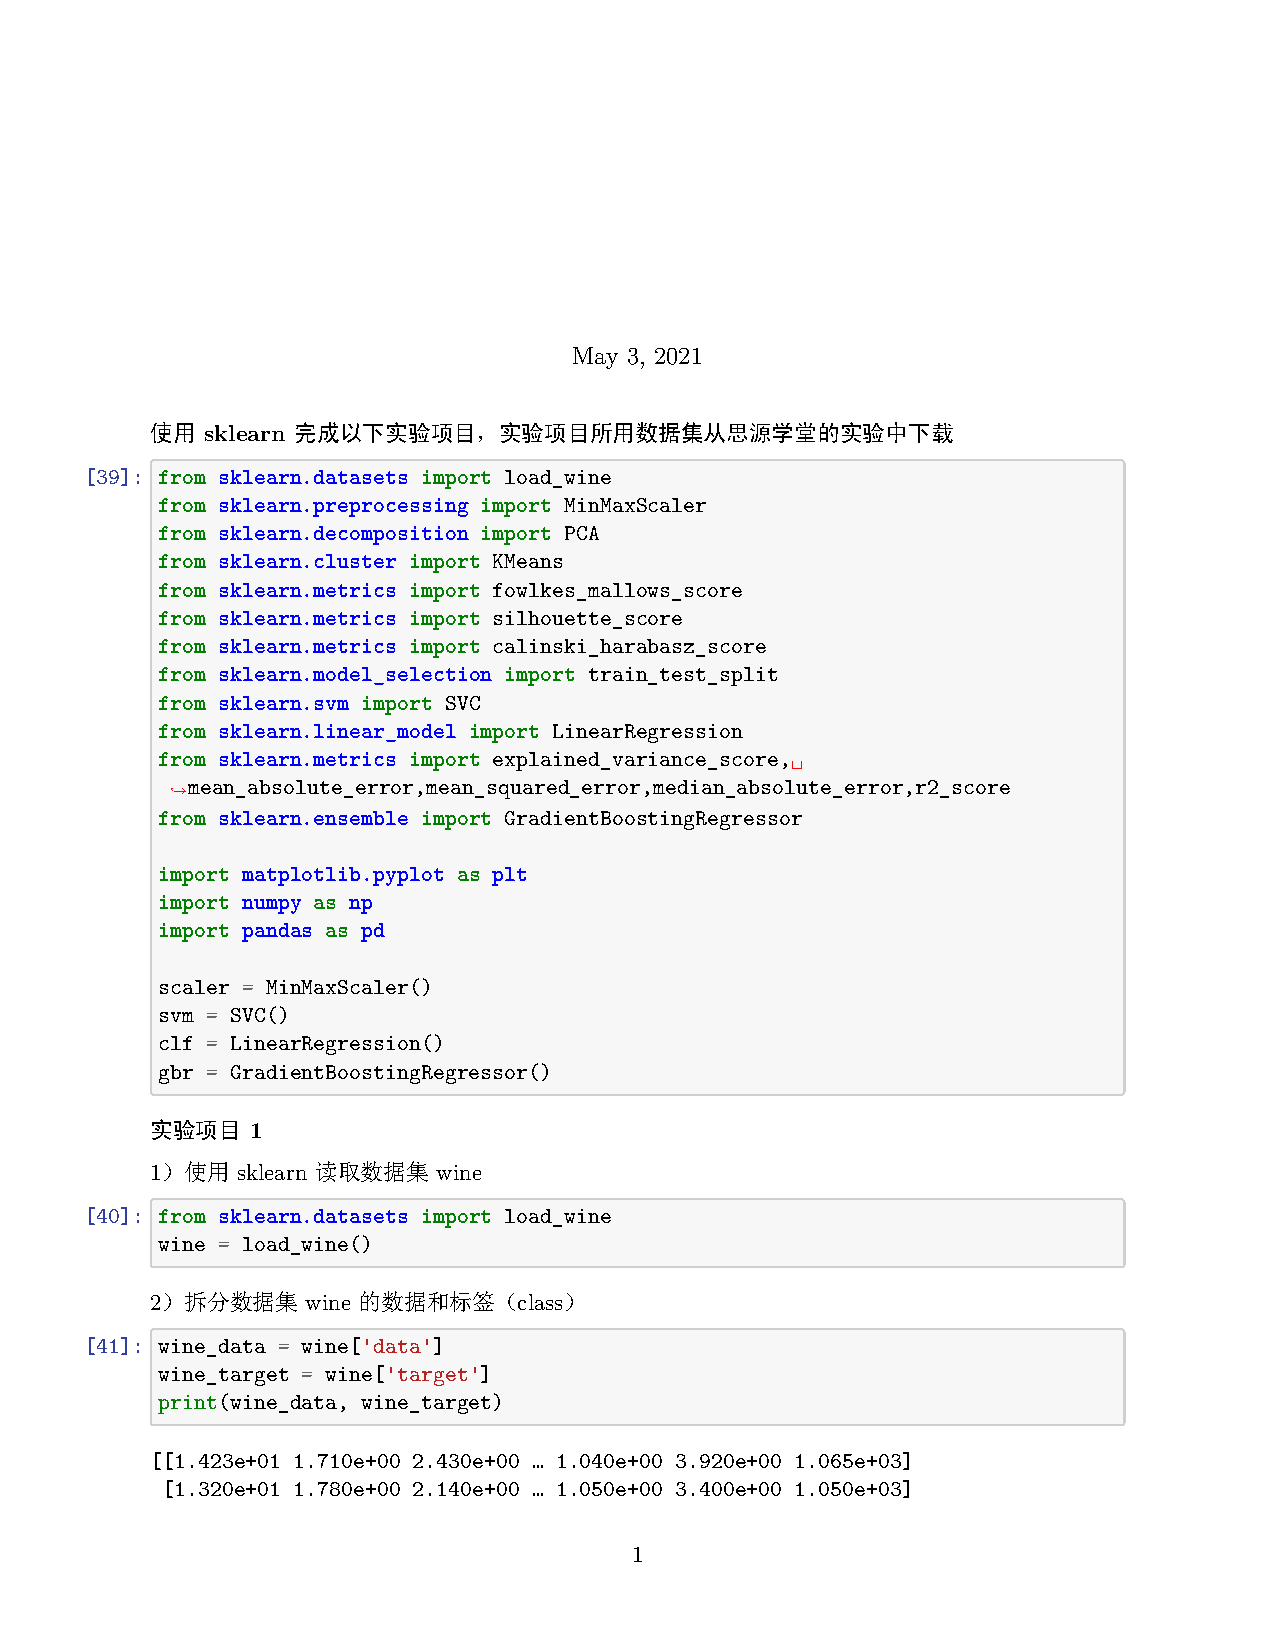
\includepdf[pages=-]{py.pdf} 

\section{code}

\subsection{Python}

\begin{lstlisting}[language=Python]
    try:
    input_arr = list(map(float, input("Please input the hetght(m) and weight(kg) number:").split()))
    if min(input_arr) < 0:
        raise Exception("The numbers should more than 0.")
    if len(input_arr) != 2:
        raise Exception("Should input 2 numbers")
except ValueError:
    print("The input is not number.")
except Exception as e:
    print(e)
else:
    BMI = input_arr[1] / input_arr[0]**2

    print("Your BMI is {0}".format(round(BMI, 1)))

    if BMI <18.5:
        print("Your body is Underweight.")
    elif BMI<23.9:
        print("Your body is Normal.")
    elif BMI<27.9:
        print("Your body is Overweight")
    else:
        print("Your body is Obesity.")

\end{lstlisting}

\subsection{R code}

\begin{lstlisting}[language=R]
    # 绘制图形
    rmax <- 3
    # 设置图形分行方式和图形空白边距,并保存原有的方式
    op <- par(mfrow = c(rmax,1), mar = .1+ c(2,2,2,1))
    for(r in 1:rmax){
      tstr <- sprintf("r=%d",r)
      ricker(0.005, r);title(tstr)
    }
    par(op) # 恢复默认图形页面设置
\end{lstlisting}

\end{document}
